
%% bare_conf.tex
%% V1.3
%% 2007/01/11
%% by Michael Shell
%% See:
%% http://www.michaelshell.org/
%% for current contact information.
%%
%% This is a skeleton file demonstrating the use of IEEEtran.cls
%% (requires IEEEtran.cls version 1.7 or later) with an IEEE conference paper.
%%
%% Support sites:
%% http://www.michaelshell.org/tex/ieeetran/
%% http://www.ctan.org/tex-archive/macros/latex/contrib/IEEEtran/
%% and
%% http://www.ieee.org/

%%*************************************************************************
%% Legal Notice:
%% This code is offered as-is without any warranty either expressed or
%% implied; without even the implied warranty of MERCHANTABILITY or
%% FITNESS FOR A PARTICULAR PURPOSE! 
%% User assumes all risk.
%% In no event shall IEEE or any contributor to this code be liable for
%% any damages or losses, including, but not limited to, incidental,
%% consequential, or any other damages, resulting from the use or misuse
%% of any information contained here.
%%
%% All comments are the opinions of their respective authors and are not
%% necessarily endorsed by the IEEE.
%%
%% This work is distributed under the LaTeX Project Public License (LPPL)
%% ( http://www.latex-project.org/ ) version 1.3, and may be freely used,
%% distributed and modified. A copy of the LPPL, version 1.3, is included
%% in the base LaTeX documentation of all distributions of LaTeX released
%% 2003/12/01 or later.
%% Retain all contribution notices and credits.
%% ** Modified files should be clearly indicated as such, including  **
%% ** renaming them and changing author support contact information. **
%%
%% File list of work: IEEEtran.cls, IEEEtran_HOWTO.pdf, bare_adv.tex,
%%                    bare_conf.tex, bare_jrnl.tex, bare_jrnl_compsoc.tex
%%*************************************************************************

% *** Authors should verify (and, if needed, correct) their LaTeX system  ***
% *** with the testflow diagnostic prior to trusting their LaTeX platform ***
% *** with production work. IEEE's font choices can trigger bugs that do  ***
% *** not appear when using other class files.                            ***
% The testflow support page is at:
% http://www.michaelshell.org/tex/testflow/



% Note that the a4paper option is mainly intended so that authors in
% countries using A4 can easily print to A4 and see how their papers will
% look in print - the typesetting of the document will not typically be
% affected with changes in paper size (but the bottom and side margins will).
% Use the testflow package mentioned above to verify correct handling of
% both paper sizes by the user's LaTeX system.
%
% Also note that the "draftcls" or "draftclsnofoot", not "draft", option
% should be used if it is desired that the figures are to be displayed in
% draft mode.
%
\documentclass[conference]{IEEEtran}
\usepackage{blindtext, graphicx}
% Add the compsoc option for Computer Society conferences.
%
% If IEEEtran.cls has not been installed into the LaTeX system files,
% manually specify the path to it like:
% \documentclass[conference]{../sty/IEEEtran}

\usepackage{enumitem}

\usepackage{subfigure}

% Some very useful LaTeX packages include:
% (uncomment the ones you want to load)


% *** MISC UTILITY PACKAGES ***
%
%\usepackage{ifpdf}
% Heiko Oberdiek's ifpdf.sty is very useful if you need conditional
% compilation based on whether the output is pdf or dvi.
% usage:
% \ifpdf
%   % pdf code
% \else
%   % dvi code
% \fi
% The latest version of ifpdf.sty can be obtained from:
% http://www.ctan.org/tex-archive/macros/latex/contrib/oberdiek/
% Also, note that IEEEtran.cls V1.7 and later provides a builtin
% \ifCLASSINFOpdf conditional that works the same way.
% When switching from latex to pdflatex and vice-versa, the compiler may
% have to be run twice to clear warning/error messages.






% *** CITATION PACKAGES ***
%
%\usepackage{cite}
% cite.sty was written by Donald Arseneau
% V1.6 and later of IEEEtran pre-defines the format of the cite.sty package
% \cite{} output to follow that of IEEE. Loading the cite package will
% result in citation numbers being automatically sorted and properly
% "compressed/ranged". e.g., [1], [9], [2], [7], [5], [6] without using
% cite.sty will become [1], [2], [5]--[7], [9] using cite.sty. cite.sty's
% \cite will automatically add leading space, if needed. Use cite.sty's
% noadjust option (cite.sty V3.8 and later) if you want to turn this off.
% cite.sty is already installed on most LaTeX systems. Be sure and use
% version 4.0 (2003-05-27) and later if using hyperref.sty. cite.sty does
% not currently provide for hyperlinked citations.
% The latest version can be obtained at:
% http://www.ctan.org/tex-archive/macros/latex/contrib/cite/
% The documentation is contained in the cite.sty file itself.






% *** GRAPHICS RELATED PACKAGES ***
%
\ifCLASSINFOpdf
  % \usepackage[pdftex]{graphicx}
  % declare the path(s) where your graphic files are
  % \graphicspath{{../pdf/}{../jpeg/}}
  % and their extensions so you won't have to specify these with
  % every instance of \includegraphics
  % \DeclareGraphicsExtensions{.pdf,.jpeg,.png}
\else
  % or other class option (dvipsone, dvipdf, if not using dvips). graphicx
  % will default to the driver specified in the system graphics.cfg if no
  % driver is specified.
  % \usepackage[dvips]{graphicx}
  % declare the path(s) where your graphic files are
  % \graphicspath{{../eps/}}
  % and their extensions so you won't have to specify these with
  % every instance of \includegraphics
  % \DeclareGraphicsExtensions{.eps}
\fi
% graphicx was written by David Carlisle and Sebastian Rahtz. It is
% required if you want graphics, photos, etc. graphicx.sty is already
% installed on most LaTeX systems. The latest version and documentation can
% be obtained at: 
% http://www.ctan.org/tex-archive/macros/latex/required/graphics/
% Another good source of documentation is "Using Imported Graphics in
% LaTeX2e" by Keith Reckdahl which can be found as epslatex.ps or
% epslatex.pdf at: http://www.ctan.org/tex-archive/info/
%
% latex, and pdflatex in dvi mode, support graphics in encapsulated
% postscript (.eps) format. pdflatex in pdf mode supports graphics
% in .pdf, .jpeg, .png and .mps (metapost) formats. Users should ensure
% that all non-photo figures use a vector format (.eps, .pdf, .mps) and
% not a bitmapped formats (.jpeg, .png). IEEE frowns on bitmapped formats
% which can result in "jaggedy"/blurry rendering of lines and letters as
% well as large increases in file sizes.
%
% You can find documentation about the pdfTeX application at:
% http://www.tug.org/applications/pdftex





% *** MATH PACKAGES ***
%
%\usepackage[cmex10]{amsmath}
% A popular package from the American Mathematical Society that provides
% many useful and powerful commands for dealing with mathematics. If using
% it, be sure to load this package with the cmex10 option to ensure that
% only type 1 fonts will utilized at all point sizes. Without this option,
% it is possible that some math symbols, particularly those within
% footnotes, will be rendered in bitmap form which will result in a
% document that can not be IEEE Xplore compliant!
%
% Also, note that the amsmath package sets \interdisplaylinepenalty to 10000
% thus preventing page breaks from occurring within multiline equations. Use:
%\interdisplaylinepenalty=2500
% after loading amsmath to restore such page breaks as IEEEtran.cls normally
% does. amsmath.sty is already installed on most LaTeX systems. The latest
% version and documentation can be obtained at:
% http://www.ctan.org/tex-archive/macros/latex/required/amslatex/math/

\usepackage[cmex10]{amsmath}
\usepackage{amsmath}
\DeclareMathOperator*{\argmax}{arg\,max}



% *** SPECIALIZED LIST PACKAGES ***
%
%\usepackage{algorithmic}
% algorithmic.sty was written by Peter Williams and Rogerio Brito.
% This package provides an algorithmic environment fo describing algorithms.
% You can use the algorithmic environment in-text or within a figure
% environment to provide for a floating algorithm. Do NOT use the algorithm
% floating environment provided by algorithm.sty (by the same authors) or
% algorithm2e.sty (by Christophe Fiorio) as IEEE does not use dedicated
% algorithm float types and packages that provide these will not provide
% correct IEEE style captions. The latest version and documentation of
% algorithmic.sty can be obtained at:
% http://www.ctan.org/tex-archive/macros/latex/contrib/algorithms/
% There is also a support site at:
% http://algorithms.berlios.de/index.html
% Also of interest may be the (relatively newer and more customizable)
% algorithmicx.sty package by Szasz Janos:
% http://www.ctan.org/tex-archive/macros/latex/contrib/algorithmicx/


\usepackage{algorithmic}

% *** ALIGNMENT PACKAGES ***
%
%\usepackage{array}
% Frank Mittelbach's and David Carlisle's array.sty patches and improves
% the standard LaTeX2e array and tabular environments to provide better
% appearance and additional user controls. As the default LaTeX2e table
% generation code is lacking to the point of almost being broken with
% respect to the quality of the end results, all users are strongly
% advised to use an enhanced (at the very least that provided by array.sty)
% set of table tools. array.sty is already installed on most systems. The
% latest version and documentation can be obtained at:
% http://www.ctan.org/tex-archive/macros/latex/required/tools/

\usepackage{array}
%\usepackage{mdwmath}
%\usepackage{mdwtab}
% Also highly recommended is Mark Wooding's extremely powerful MDW tools,
% especially mdwmath.sty and mdwtab.sty which are used to format equations
% and tables, respectively. The MDWtools set is already installed on most
% LaTeX systems. The lastest version and documentation is available at:
% http://www.ctan.org/tex-archive/macros/latex/contrib/mdwtools/


% IEEEtran contains the IEEEeqnarray family of commands that can be used to
% generate multiline equations as well as matrices, tables, etc., of high
% quality.


%\usepackage{eqparbox}
% Also of notable interest is Scott Pakin's eqparbox package for creating
% (automatically sized) equal width boxes - aka "natural width parboxes".
% Available at:
% http://www.ctan.org/tex-archive/macros/latex/contrib/eqparbox/





% *** SUBFIGURE PACKAGES ***
%\usepackage[tight,footnotesize]{subfigure}
% subfigure.sty was written by Steven Douglas Cochran. This package makes it
% easy to put subfigures in your figures. e.g., "Figure 1a and 1b". For IEEE
% work, it is a good idea to load it with the tight package option to reduce
% the amount of white space around the subfigures. subfigure.sty is already
% installed on most LaTeX systems. The latest version and documentation can
% be obtained at:
% http://www.ctan.org/tex-archive/obsolete/macros/latex/contrib/subfigure/
% subfigure.sty has been superceeded by subfig.sty.

\usepackage{graphicx}
\usepackage[caption=false]{caption}
\usepackage{subcaption}
% subfig.sty, also written by Steven Douglas Cochran, is the modern
% replacement for subfigure.sty. However, subfig.sty requires and
% automatically loads Axel Sommerfeldt's caption.sty which will override
% IEEEtran.cls handling of captions and this will result in nonIEEE style
% figure/table captions. To prevent this problem, be sure and preload
% caption.sty with its "caption=false" package option. This is will preserve
% IEEEtran.cls handing of captions. Version 1.3 (2005/06/28) and later 
% (recommended due to many improvements over 1.2) of subfig.sty supports
% the caption=false option directly:
%\usepackage[caption=false,font=footnotesize]{subfig}
%
% The latest version and documentation can be obtained at:
% http://www.ctan.org/tex-archive/macros/latex/contrib/subfig/
% The latest version and documentation of caption.sty can be obtained at:
% http://www.ctan.org/tex-archive/macros/latex/contrib/caption/




% *** FLOAT PACKAGES ***
%
%\usepackage{fixltx2e}
% fixltx2e, the successor to the earlier fix2col.sty, was written by
% Frank Mittelbach and David Carlisle. This package corrects a few problems
% in the LaTeX2e kernel, the most notable of which is that in current
% LaTeX2e releases, the ordering of single and double column floats is not
% guaranteed to be preserved. Thus, an unpatched LaTeX2e can allow a
% single column figure to be placed prior to an earlier double column
% figure. The latest version and documentation can be found at:
% http://www.ctan.org/tex-archive/macros/latex/base/



%\usepackage{stfloats}
% stfloats.sty was written by Sigitas Tolusis. This package gives LaTeX2e
% the ability to do double column floats at the bottom of the page as well
% as the top. (e.g., "\begin{figure*}[!b]" is not normally possible in
% LaTeX2e). It also provides a command:
%\fnbelowfloat
% to enable the placement of footnotes below bottom floats (the standard
% LaTeX2e kernel puts them above bottom floats). This is an invasive package
% which rewrites many portions of the LaTeX2e float routines. It may not work
% with other packages that modify the LaTeX2e float routines. The latest
% version and documentation can be obtained at:
% http://www.ctan.org/tex-archive/macros/latex/contrib/sttools/
% Documentation is contained in the stfloats.sty comments as well as in the
% presfull.pdf file. Do not use the stfloats baselinefloat ability as IEEE
% does not allow \baselineskip to stretch. Authors submitting work to the
% IEEE should note that IEEE rarely uses double column equations and
% that authors should try to avoid such use. Do not be tempted to use the
% cuted.sty or midfloat.sty packages (also by Sigitas Tolusis) as IEEE does
% not format its papers in such ways.





% *** PDF, URL AND HYPERLINK PACKAGES ***
%
%\usepackage{url}
% url.sty was written by Donald Arseneau. It provides better support for
% handling and breaking URLs. url.sty is already installed on most LaTeX
% systems. The latest version can be obtained at:
% http://www.ctan.org/tex-archive/macros/latex/contrib/misc/
% Read the url.sty source comments for usage information. Basically,
% \url{my_url_here}.





% *** Do not adjust lengths that control margins, column widths, etc. ***
% *** Do not use packages that alter fonts (such as pslatex).         ***
% There should be no need to do such things with IEEEtran.cls V1.6 and later.
% (Unless specifically asked to do so by the journal or conference you plan
% to submit to, of course. )


% correct bad hyphenation here
\hyphenation{op-tical net-works semi-conduc-tor}


\begin{document}
%
% paper title
% can use linebreaks \\ within to get better formatting as desired
\title{Predicting Income Level for Adults in the United States}


% author names and affiliations
% use a multiple column layout for up to three different
% affiliations
\author{\IEEEauthorblockN{Sung-Li Chiang}
\IEEEauthorblockA{Mechanical Engineering\\ University of California, Berkeley\\
Email: slchiang@berkeley.edu \\ 
SID: 24978880}
\and
\IEEEauthorblockN{Dennis Wai}
\IEEEauthorblockA{Mechanical Engineering\\ University of California, Berkeley\\
Email: dwai213@berkeley.edu \\ 
SID: 21183965}
}

% conference papers do not typically use \thanks and this command
% is locked out in conference mode. If really needed, such as for
% the acknowledgment of grants, issue a \IEEEoverridecommandlockouts
% after \documentclass

% for over three affiliations, or if they all won't fit within the width
% of the page, use this alternative format:
% 
%\author{\IEEEauthorblockN{Michael Shell\IEEEauthorrefmark{1},
%Homer Simpson\IEEEauthorrefmark{2},
%James Kirk\IEEEauthorrefmark{3}, 
%Montgomery Scott\IEEEauthorrefmark{3} and
%Eldon Tyrell\IEEEauthorrefmark{4}}
%\IEEEauthorblockA{\IEEEauthorrefmark{1}School of Electrical and Computer Engineering\\
%Georgia Institute of Technology,
%Atlanta, Georgia 30332--0250\\ Email: see http://www.michaelshell.org/contact.html}
%\IEEEauthorblockA{\IEEEauthorrefmark{2}Twentieth Century Fox, Springfield, USA\\
%Email: homer@thesimpsons.com}
%\IEEEauthorblockA{\IEEEauthorrefmark{3}Starfleet Academy, San Francisco, California 96678-2391\\
%Telephone: (800) 555--1212, Fax: (888) 555--1212}
%\IEEEauthorblockA{\IEEEauthorrefmark{4}Tyrell Inc., 123 Replicant Street, Los Angeles, California 90210--4321}}




% use for special paper notices
%\IEEEspecialpapernotice{(Invited Paper)}




% make the title area
\maketitle
\thispagestyle{plain}
\pagestyle{plain}

\begin{abstract}
In this report, we implemented both parametric and non-parametric machine learning techniques. We compared the results  of perceptron, decision tree, logistic regression and neural network. In addition, we added L1 norm regularization to the latter two methods to regularize our model parameters. We also extended basic algorithms by either further generalizing them (ex. $n$ hidden layer neural network) or improving the technique's short-comings (ex. depth-limited decision trees). Finally, we used L1 regularization as a means for feature selection to identify influential features for income prediction.
\end{abstract}
% IEEEtran.cls defaults to using nonbold math in the Abstract.
% This preserves the distinction between vectors and scalars. However,
% if the journal you are submitting to favors bold math in the abstract,
% then you can use LaTeX's standard command \boldmath at the very start
% of the abstract to achieve this. Many IEEE journals frown on math
% in the abstract anyway.

% Note that keywords are not normally used for peerreview papers.
% \begin{IEEEkeywords}
% IEEEtran, journal, \LaTeX, paper, template.
% \end{IEEEkeywords}

% For peer review papers, you can put extra information on the cover
% page as needed:
% \ifCLASSOPTIONpeerreview
% \begin{center} \bfseries EDICS Category: 3-BBND \end{center}
% \fi
%
% For peerreview papers, this IEEEtran command inserts a page break and
% creates the second title. It will be ignored for other modes.
\IEEEpeerreviewmaketitle

\section{Introduction}
\subsection{Objective}
In this work, we will investigate the use of four different classifiers (two parametric, two non-parametric) in income level prediction. In particular, we will be using perceptron, decision trees, the logistic regression framework, and neural networks to predict if a particular adult will make more than 50K a year. Our preliminary work using standard SVM (Fig. \ref{fig:svm}) and nearest neighbor (Fig. \ref{fig:nearestNeighbor}) informed us that the data is complex and highly probable to be linearly inseparable. For that reason, we forecast that techniques like perceptron and logistic regression, which assumes that the data fits a linear model, to be on par with SVM and have mediocre prediction performance. Therefore, we project that non-parametric methods such as decision trees and neural networks, which can represent more complex models, to achieve better prediction performance. \\
Moreover, we will use L1-regularization when applicable to perform feature selection. Because of the real world applicability, we think it will be interesting and informative to use a machine learning based approach to identify influential factors in adult income level.
\begin{figure}[h!]
\centering
\includegraphics[width=3in]{svm.jpg}
\caption{Results of a SVM classifier on two features, age and hours-per-week. The prediction accuracy was 76.05\%.}
\label{fig:svm}
\end{figure}
\begin{figure}[h!]
\centering
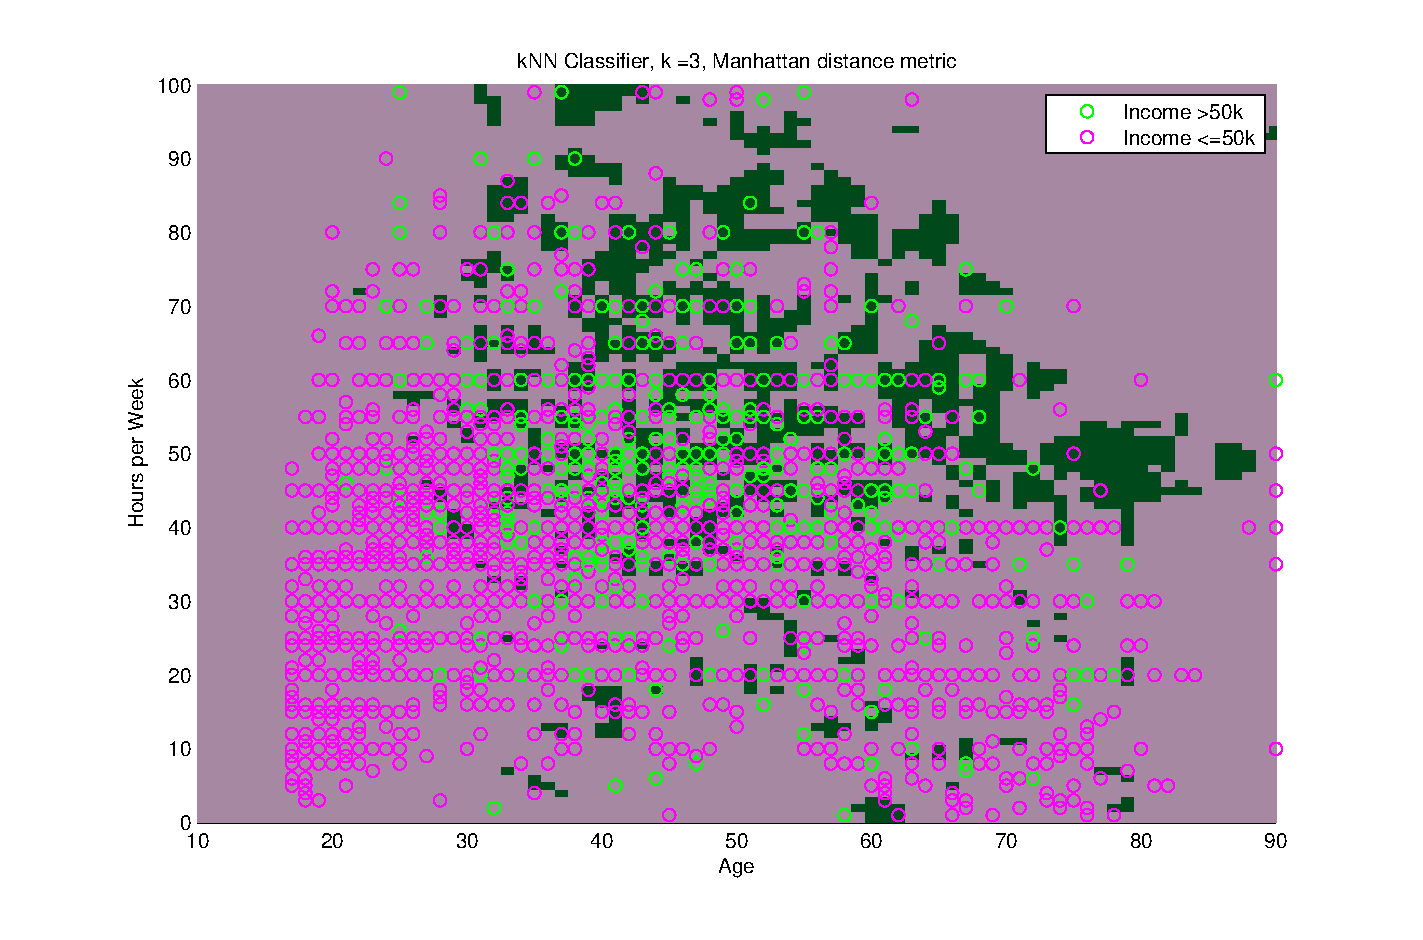
\includegraphics[width=3in]{nearestNeighbor.eps}
\caption{Results of a kNN ($k=3$, Manhattan distance metric) classifier on two features (age and hours-per-week). The dark green patches represent the classifier’s decision region in which the classifier will classify the data as green ($>$50K). The prediction accuracy was 71\%}
\label{fig:nearestNeighbor}
\end{figure}
\subsection{Adult Dataset}
The adult dataset can be freely downloaded at \cite{UCI} and contains both a training and test set. The training set has 32561 samples while the test set has 16281 samples. The dataset is aggregated from the results of the 1994 census data. Each training and testing sample also comes with a label of +1 and 0, which corresponds to $>$50K and $<=$50K, respectively. There are 14, 2 of which superfluous, features used for this study. The 12 features are:
\begin{itemize}
    \item Age: The age of the respondee
    \item Workclass: The workclass of the respondee (ex. private employed, state government employed)
    \item Education: The education lavel of the respondee (ex. Bachelors, Doctorate)
    \item Marital-Status: The marital status of the respondee (ex. Widowed, separated)
    \item Occupation: The respondee occupation (ex. Sales, armed-forces)
    \item Relationship: The respondee's relationship status (ex. wife, unmarried)
    \item Race: The respondee's race (ex. white, black)
    \item Sex: The respondee's gender
    \item Capital-Gain: The respondee's capital-gain
    \item Capital-Loss: The respondee's capital-loss
    \item Hours-per-week: The respondee's hours at work per week
    \item Native-Country: The respondee's country of origin (ex. Vietnam, Mexico)
\end{itemize}
For a full listing of each feature's options, please refer to \cite{UCI} for full details.
\section{Implementation}
\subsection{Parametric Approach}
% \begin{enumerate}
\subsubsection{ Perceptron with MIRA (Margin Infused Relaxed Algorithm)} 
The multiclass perceptron classifier is a simple and lightweight machine learning technique. In this classifier, there are $n$ weights for the $n$ classes to be classified. (In our case, $n = 2$). These $n$ weights ($w_i \ \ \ \forall i \in [1, \,n]$) are randomly initialized $\sim\mathcal{N}(0,.1)$ and are of dimension $\mathcal{R}^{d+1}$, where $d$ is the number of features per sample and the $1$ is for better generality. These weights are then updated in training time until each weight represent a half plane's normal vector that can sufficiently classify data points. The pseudocode is provided below:
\begin{enumerate}
    \item Randomly initialize weight
    \item Select randomly a training sample
    \item Choose prediction to be the $\underset{y}{\operatorname{argmax}} \quad w_i \cdot f(x)$
    \item If prediction was correct, then don't change the weights
    \item If prediction was incorrect then update the weights 
    \begin{enumerate}
        \item $w_i = w_i - f(x)$
        \item $w_{i^*} = w_{i^*} + f(x)$ \\
        where $w_{i^*}$ denotes the correct class, $w_i$ the incorrectly predicted class, and $f(x)$ is the data point
    \end{enumerate}
\end{enumerate} 
The astute student will observe that in linearly non-separable data, this algorithm will never converge. For that reason, we defined convergence to be the point in which training accuracy remained stagnant within a tuned tolerance, $\epsilon$. \\
To facilitate convergence, we borrowed an idea from CS188 and implemented the MIRA variant of perceptron algorithm. Largely similar to the standard multiclass perceptron, the MIRA perceptron adds a learning rate term to the update equation (i.e. $w_{i^*} = w_{i^*} + \tau f(x)$. The prescription for $\tau$ is:
\begin{align*}
  \tau = \min{\left(\frac{(w_{i} - w_{i^*})\cdot f}{2 f \cdot f},C\right)}
\end{align*}
where $C$ is a tunable hyperparameter that reflects the maximum allowable learning rate and $w_{i^*}$ and $w_i$ are as previously defined.
\subsubsection{ Logistic Regression with L1 Norm Regularization}
First, we assume that data of different classes share the same covariance but have different means. Then, we define the loss function as a function of learning parameter $\beta$ as follows:
\begin{center}
\begin{equation}
l(\beta) = \lambda\|\beta\|_1-\sum_{i=1}^n [ y_i \textit{log} \mu_i + (1-y_i)\textit{log}(1-\mu_i) ]
\end{equation}
\end{center}
where $\mu_i(\beta)=1/(1+\text{exp}(-\beta^Tx_i))$ is a logistic function, and $\lambda>0$ is a tunable regularization parameter. L1 norm is used as the loss function to enforce sparsity and to select informative features.\\
To perform logistic regression, first randomly initialize $\beta$ and then use stochastic gradient descent. Iteratively perform the gradient descent while updating the parameter $\beta$. $\beta$ will then gradually converge to the optimal value and then stop once the the stopping criterion is satisfied. The gradient of the loss function with respect to $\beta$ (Eq. \ref{eqn:gradient}) and the update equation (Eq. \ref{eqn:update}) are shown below: \\
\begin{align}
\nabla_\beta l(\beta) &=  \lambda \text{sign}(\beta)-[y_i-\mu_i(\beta)]*x_i  \label{eqn:gradient} \\
\beta &= \beta-\eta*\nabla_\beta l(\beta) \label{eqn:update}
\end{align}
where $\eta$ is the learning rate, a hyper-parameter is tuned by cross validation.\\
The stopping criterion in this implementation is either the algorithm iteration count exceeds a fixed amount or if the difference in the loss between two sequential iteration is less than a tuned threshold, $\epsilon$.
% \end{enumerate}

\subsection{Non-Parametric Approach}
% \begin{enumerate}
\subsubsection{ Decision Tree} 
This method is an example of a non-parametric algorithm that can easily be extended to ensemble methods. In our implementation, we used cross validation to set a maximum tree depth of 10 ($d=10$). Moreover, we used the standard information gain (Eq. \ref{eq:informationGain}) and entropy function (Eq. \ref{eq:entropy}) to enable the tree to make splits at each layer. For each tree, the optimal splits are learned according to the pseudocode in Fig. \ref{fig:treeLearningAlgo}.
\begin{align}
IG &= H(\text{parent}) - \frac{1}{N}\sum_i^N H(\text{children}) \label{eq:informationGain} \\
H &= \sum_i -p_i \log{p_i}_2 \label{eq:entropy}
\end{align}
Because the adult dataset has a low amount of features, the decision trees are easy to train. With the depth limited to 10, these trees naturally become weak learners as well. For these reasons, we naturally extended decision trees to random forest to take advantage of the benefits of ensemble learning techniques, which include robustness to noise and avoiding model over fitting. In our implementation, we chose a tree depth limit of 10, splitting only on 4 randomly features at each layer, and used 100 trees in the forest.
\begin{figure}[h!]
\centering
\includegraphics[width=3.5in]{treeLearningAlgo.png}
\caption{Pseudocode for decision tree learning, reproduced from CS289A lecture slides}
\label{fig:treeLearningAlgo}
\end{figure} \\
\subsubsection{ Neural Network with Multiple Layers}
In neural network design, we focused on using mean-squared error and cross-entropy error function to train our multi-layered nets ($>$2) and different number of hidden nodes. The hidden layers' activation functions are hyperbolic tangent of input signal ($\tanh{(x)}$) and output layer's activation function is the sigmoid function ($g(x)=\frac{1}{1+\text{exp}(-x)}$).\\
The training algorithm is implemented as follows:\\
\begin{enumerate}
\item Randomly initialize all weights,$w_{ij}$ uniformly distributed in $[-\epsilon,\epsilon]$ where $\epsilon>0$ is a small number.\\ 
\item Compute all $x_i^{l}$ through forward propagation\\
\begin{itemize}
\item For hidden layers:
\begin{center}
\begin{align}
s_j^{(l+1)} = \sum_{i}w_{ij}^{(l+1)}*x_i^{(l)}\\
x_j^{(l+1)} = \text{tanh}(s_j^{(l+1)})
\end{align}
\end{center}
where $s_j^{(l+1)}$ is the input of $j$-th node in $(l+1)$-th layer, and $x_j^{(l+1)}$ is the output of $j$-th node in $(l+1)$-th layer .\\
\item For output layer:
\begin{center}
\begin{align}
s_j^{(L)} = \sum_{i}w_{ij}^{(L)}*x_i^{(L-1)}\\
x_j^{(L)} = \text{tanh}(s_j^{(L)})
\end{align}
\end{center}
where $s_j^{(L)}$ is the input of $j$-th node in output layer, and $x_j^{(L)}$ is the output of $j$-th node in output layer .\\
\end{itemize}
\item Backward compute all $\delta_j^{(l)}$ where $\delta_j^{(l)}=\frac{\partial J}{\partial s_j^{(l)}}$ and J is the mean-squared error or cross-entropy error function (with or without L1 norm regularization). The following shows the cross-entropy error as an example of loss function:
\begin{center}
\begin{align} \nonumber
J = -\sum_{k=1}^{n_out}[y_k \text{ln} (g(s_k^{(L)}))+(1-y_k) \text{ln} (1-g(s_k^{(L)}))\\
+ \left( \lambda \|w_{ij}^{(1)} \|_1 \right)]   
\end{align}
\end{center}
\begin{itemize}
\item For output layer:
\begin{center}
\begin{align}
\frac{\partial J}{\partial w_{ij}^{(L)}} &= \frac{\partial J}{\partial s_{j}^{(L)}}\frac{\partial s_{j}^{(L)}} {\partial w_{ij}^{(L)}}\\
&= \delta_j^{(L)}x_i^{(L-1)}\\
&= g(s_{j}^{(L)})(1-g(s_{j}^{L}))(g(s_{j}^{(L)})-y_j)x_i^{(L-1)}
\end{align}
\end{center}
\item For hidden layers:\\
\begin{center}
\begin{align}
\frac{\partial J}{\partial w_{ij}^{(l)}} &= \frac{\partial J}{\partial s_{j}^{(l)}}\frac{\partial s_{j}^{(l)}} {\partial w_{ij}^{(l)}}\\
&= \delta_j^{(l)}x_i^{(l-1)}\\
&= \sum_{k=1}^{d(l+1)}\frac{\partial J}{\partial s_k^{(l+1)}}\frac{\partial s_k^{(l+1)}}{\partial x_j^{(l)}}\frac{\partial x_j^{(l)}}{\partial s_j^{(l)}}x_i^{(l-1)}\\
&= \sum_k(\delta_k^{(l+1)})(w_{jk}^{(l+1)})(\frac{\partial \text{tanh}(s_j^{(l)})}{\partial s_j^{(l)}})x_i^{(l-1)}
\end{align}
\end{center}
\end{itemize}
where $k$ is the node in next layer and $d^{(l+1)}$ is the number of nodes in the next layer.
\item Update weights\\
\begin{center}
\begin{align}
w_{ij}^{(l)} &=  w_{ij}^{(l)} - \eta \frac{\partial J}{\partial w_ij^{(l)}}\\ 
&= w_{ij}^{(l)} - \eta x_i^{(l-1)}\delta_j^{l}
\end{align}
\end{center}
where $\eta$ is the learning rate selected through cross validation. 
\item Repeat step 2 to 4 until the difference between old loss and new loss is less than a small number or the iteration time higher than a big number. \\
\begin{figure}[hb]
\centering
\includegraphics[scale=0.3]{nn.jpg}
\caption{Neural network structure}
\label{fig:nn}
\end{figure}
\end{enumerate}

% \end{enumerate}

\section{Results and Analysis} \label{result}

\subsection{Logistic Regression}
For the logistic regression method, we compare the accuracy of using L1 norm regularization and without. In addition, we can seek out the most influential features by inducing sparsity through the inclusion of an L1 norm in the loss function. The four features with highest weight magnitude are capital-gain, education level, marital-status and the age of the person who takes the survey.\\
This method's prediction accuracy are shown in Table \ref{table:log}. Note that the selected features used in this trial were education and marital status. 
\begin{table}[h]
\centering
\begin{tabular}{|c|c|}
\hline
                              & \textbf{Testing Accuracy} \\ \hline
\textbf{All features}          & 83.94\%                      \\ \hline
\textbf{All features + L1 norm} & 83.71\%                      \\ \hline
\textbf{Selected feature}     & 76.14\%                      \\ \hline
\end{tabular}
\caption{Prediction Accuracy of Logistic Regression}
\label{table:log}
\end{table}\\
In Table \ref{table:log}, the accuracy from logistic regression with selected features(education and marital-status) is an impressive $76.14\%$ because those features give us a sufficiently good prediction rates. Furthermore, including the remaining 11 features only marginally improve the accuracy by less than 10 percent. As for logistic regression with L1 norm, the accuracy is $83.71 \%$, which is slightly worse compared to the un-regularized logistic regression classifier trained with all of the features. Even though L1 norm regularization leads to a sparse $\beta$ that leaves certain features unused, the algorithm performs adequately well on our test data set.\\ 

\subsection{Neural Network}
In Figures \ref{fig:W1},\ref{fig:L1MSE},\ref{fig:L1CE}, we visualize the weights that connect the input layer to the first hidden layer of the neural network. In Fig. \ref{fig:W1}, we trained a standard neural net and the visualization demonstrate that each input feature connects to many of the hidden nodes with a significant amount of activation. Note that the 12th feature (capital loss) has a relatively larger activation than the other features. However in Fig. \ref{fig:L1MSE} and Fig. \ref{fig:L1CE}, which includes a L1 loss in the loss function, it is clear that the 6th, 7th and 12th features(education, marital-status and capital loss, respectively) are the most influential features. In contrast, the other input features nodes are largely deactivated. \\
\begin{figure}
\begin{subfigure}{\linewidth}
\includegraphics[scale=0.4]{W1all.jpg}
\caption{Weights of the first layer with all features}\label{fig:W1}
\end{subfigure}%
\begin{subfigure}{\linewidth}
\includegraphics[scale=0.4]{L1MSE.jpg}
\caption{Weights for the first layer subjected to L1 regularization with MSE}\label{fig:L1MSE}
\end{subfigure}%
\begin{subfigure}{\linewidth}
\includegraphics[scale=0.4]{L1CE.jpg}
\caption{Weights subjected to L1 regularization with cross-entropy loss}\label{fig:L1CE}
\end{subfigure}%
\end{figure}
The results in Table \ref{table:nnets} show that the neural network with multiple hidden layers doesn't perform as well as the neural network with a single hidden layer. One possible reason for the error may be attributed to the random weight initialization before training and both neural networks are actually providing an equivalent prediction accuracy. Alternatively, the number of nodes in the extra hidden layer is not large enough to distinguish each network from another. Another reason might be multiple layers networks might overfit the training data so that the network performs poorly on the test data.\\
On the other hand, the neural network's performance with reduced but manually selected features (education and marital-status) is comparable to the neural network trained with all of the features. This suggests that these two particular features can actually give us a lot of information when it comes to income level prediction. In the real world, people with a higher education level typically have a higher chance to earn more money. Also, people who are single might choose to have stressful jobs that produce a higher personal income. But when people are married, the same people might choose jobs with more flexible hours, at the cost of less income, so that they can spend more time with their family.\\ 

\begin{table}[h]
\centering
\begin{tabular}{|c|c|c|}
\hline
                                   & \textbf{Mean-Square Error} & \textbf{Cross-Entropy Error} \\ \hline
$\mathbf{n_{hid}=200}$               & 84.42\%                    & 84.37\%                      \\ \hline
$\mathbf{n_{hid1}=300 \ n_{hid2}=100}$    & 84.37\%                    & 84.23\%                      \\ \hline
$\mathbf{n_{hid}=200 \textbf{ with L1}}$             & 84.23\%                    & 84.15\%                      \\ \hline
$\mathbf{n_{hid}=200 \textbf{ and selected Feat.}}$ & 83.38\%                    & 82.38\%                      \\ \hline
\end{tabular}
\caption{Neural network accuracy with different loss functions. $\mathbf{n_{hid}}$ is the node number in the hidden layer}
\label{table:nnets}
\end{table}

\subsection{Decision Tree}
We ran four variants of the decision tree algorithm and the classification results are presented in Table. \ref{table:treesResults}.
\begin{table}[h]
\centering
\begin{tabular}{|c|c|}
\hline
\textbf{Method} & \textbf{Testing Accuracy} \\ \hline
\textbf{Decision Tree} & 82.10\% \\ \hline
\textbf{Decision Tree, $d$ = 10} & 85.18\% \\ \hline
\textbf{Random Forest} & 84.90\% \\ \hline
\textbf{Random Forest, $d$ = 10} & 85.76\% \\ \hline
\end{tabular}
\caption{Table of classification results for the decision tree algorithm. Here $d$ refers to the tree's maximum depth}
\label{table:treesResults}
\end{table} \\
From the first two rows in Table. \ref{table:treesResults}, we can clearly see that preventing the tree from growing beyond a depth of $d$ prevents overfitting and improves prediction accuracy. The $d$ was chosen empirically through cross validation. Moreover, the last two rows in Table \ref{table:treesResults} demonstrate the benefits of the ensemble learning technique, random forest. The significant increase in prediction accuracy can be attributed to noise rejection as well as a decrease in model over fitting. For example trees ($d=4$) used in our random forest, please refer to Fig. \ref{fig:visualTree} in the Appendix. \\
Similar to what was done for neural nets and logistic regression, we performed a pseudo L1 regularization with decision trees by creating 300 trees and counting the occurrences of the top level split as a mechanism for feature selection. The results are presented in Table: \ref{table:occurTree}
\begin{table}[h]
\centering
\begin{tabular}{|c|c|}
\hline
\textbf{Feature} & \textbf{Occurrence as Top Split in 300 Trees} \\ \hline
\textbf{age} & 72 \\ \hline
\textbf{workclass} & 73 \\ \hline
\textbf{education} & 71 \\ \hline
\textbf{marital-status} & 84 \\ \hline
\end{tabular}
\caption{Table of the occurrences of a particular feature as the top level split out of 300 decision trees.}
\label{table:occurTree}
\end{table}
\\
Table \ref{table:occurTree} demonstrates that out of the 12 possible features, only four features are ever used as the top level split: age, workclass, education (education-num), and marital status. Because this result overlaps with the features selected by L1 regularization in other methods, these four features are relatively more influential in determining the income level of adults. \\
\subsection{Perceptron}
We ran three variants of the perceptron algorithm and the results are presented in Table \ref{table:perceptronResults}.
\begin{table}[h]
\centering
\begin{tabular}{|c|c|}
\hline
\textbf{Method} & \textbf{Testing Accuracy} \\ \hline
\textbf{Perceptron} & 78.340\% \\ \hline
\textbf{Perceptron with MIRA} & 79.140\% \\ \hline
\textbf{Perceptron with MIRA and reduced features} & 76.340\% \\ \hline
\end{tabular}
\caption{Table of Testing Accuracy for the Perceptron algorithm and its variants}
\label{table:perceptronResults}
\end{table} \\
From Table \ref{table:perceptronResults}, it is clear that the perceptron with MIRA offered slightly superior prediction accuracy, which can be explained by the adaptive learning rate prescribed by MIRA. From the L1-regularization results presented before, we decided to run the perceptron algorithm again but on a reduced dimension data set. We chose to train and predict on a dataset that only included education and marital status information. The classification result is presented in Fig. \ref{fig:miraPerceptron}. 
\begin{figure}[h!]
\centering
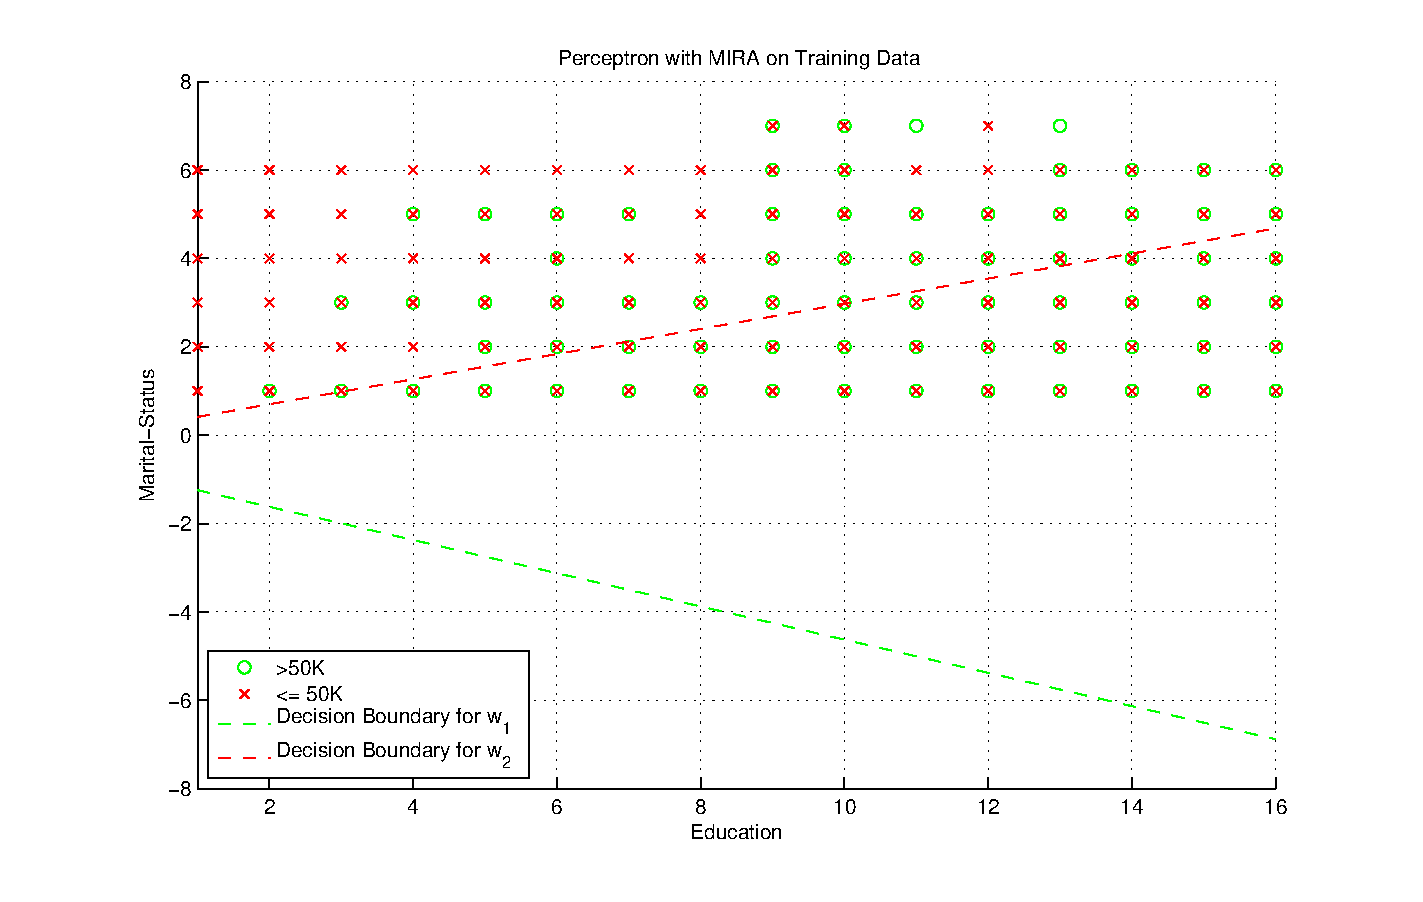
\includegraphics[width=3.5in]{miraPerceptron.eps}
\caption{Plot of the two hyperplanes computed by the perceptron with MIRA. $w_1$ represents the weight vector for data points with positive labels ($>$50K).}
\label{fig:miraPerceptron}
\end{figure}

% \end{enumerate}
\section{Conclusion}
Section \ref{result} showed that no a priori assumptions can be made in regards to what machine learning technique is best for classification. We initially believed that neural network would have been the most accurate technique but was proved wrong when random forests proved to be marginally more accurate. However, we do recognize that tuning hyperparameters, such as the learning rate in a neural network, can drastically affect the performance of a classifier. Therefore, the poor prediction accuracy does not necessarily indicate a limitation of the technique but potentially rather a lack of finesse in the art of tuning. \\
Through our L1-regularization in neural networks and logistic regression as well as counting the occurrences of top-level splits in decision tree, we concluded that education and marital status are the most influential features for classification. Using only these features, we showed that classifiers trained with these features can still achieve respectable prediction accuracy. Education and marital status are also validated from real world experiences because in general having a higher education tends to lead to better paying jobs that can provide an income more than 50K. We conclude, however, that the aforementioned features are not definitive in income level prediction. There are various complicated relationships that intricately tie all of the features as well as many external factors that are not captured within the dataset.

% if have a single appendix:
%\appendix[Proof of the Zonklar Equations]
% or
%\appendix  % for no appendix heading
% do not use \section anymore after \appendix, only \section*
% is possibly needed

% use appendices with more than one appendix
% then use \section to start each appendix
% you must declare a \section before using any
% \subsection or using \label (\appendices by itself
% starts a section numbered zero.)
%


\appendices
\section{Decision Tree Visualization}
In this section, we present a visualization of a depth limited tree used in our random forests. Note that in the interest of brevity, we set $d=4$ for this example tree. Otherwise, each node in the tree can be interpreted by reading the split rule as well as the amount of positive and negative samples in the node. For example, the top node splits on whether the data sample has a marital status that is less than 1.81.
\begin{figure}[h!]
\centering
\includegraphics[width=3.5in]{visualTree.png}
\caption{Visualization of a typical decision tree used in a random forest. Note that for visual brevity, this tree has $d=4$ instead of $d=10$.}
\label{fig:visualTree}
\end{figure}
\begin{figure}[h!]
\centering
\includegraphics[width=3.5in]{visualTree2.png}
\caption{Visualization of a typical decision tree used in a random forest. This tree's top split is education level}
\label{fig:visualTree2}
\end{figure}

\section{Report Code}
For a downloadable version of the code used to reproduce this work, please go to \text{https://github.com/dwai213/ML_census}

% use section* for acknowledgement
\section*{Acknowledgment}
The authors would like to thank the CS289A teaching staff for their continued hard work in machine learning education as well as the UC Irvine Machine Learning repository for their readily downloadable datasets.

% Can use something like this to put references on a page
% by themselves when using endfloat and the captionsoff option.
\ifCLASSOPTIONcaptionsoff
  \newpage
\fi

% trigger a \newpage just before the given reference
% number - used to balance the columns on the last page
% adjust value as needed - may need to be readjusted if
% the document is modified later
%\IEEEtriggeratref{8}
% The "triggered" command can be changed if desired:
%\IEEEtriggercmd{\enlargethispage{-5in}}

% references section

% can use a bibliography generated by BibTeX as a .bbl file
% BibTeX documentation can be easily obtained at:
% http://www.ctan.org/tex-archive/biblio/bibtex/contrib/doc/
% The IEEEtran BibTeX style support page is at:
% http://www.michaelshell.org/tex/ieeetran/bibtex/
%\bibliographystyle{IEEEtran}
% argument is your BibTeX string definitions and bibliography database(s)
%\bibliography{IEEEabrv,../bib/paper}
%
% <OR> manually copy in the resultant .bbl file
% set second argument of \begin to the number of references
% (used to reserve space for the reference number labels box)
\begin{thebibliography}{1}

\bibitem{UCI}
UCI Machine Learning Repository:http://archive.ics.uci.edu/ml/datasets/Adult
\bibitem{UScensus}
United States Census Bureau: http://www.census.gov/hhes/www/income/data/index.html
\bibitem{cs188}
Lecture slides from Spring 2015 taught by Pieter Abbeel
\bibitem{cs289a}
Lecture slides from Spring 2015 taught by Alexi Efros and Peter Bartlett 
\end{thebibliography}

% biography section
% 
% If you have an EPS/PDF photo (graphicx package needed) extra braces are
% needed around the contents of the optional argument to biography to prevent
% the LaTeX parser from getting confused when it sees the complicated
% \includegraphics command within an optional argument. (You could create
% your own custom macro containing the \includegraphics command to make things
% simpler here.)
%\begin{biography}[{\includegraphics[width=1in,height=1.25in,clip,keepaspectratio]{mshell}}]{Michael Shell}
% or if you just want to reserve a space for a photo:

\begin{IEEEbiography}[{\includegraphics[width=1in,height=1.25in,clip,keepaspectratio]{picture}}]{John Doe}
\blindtext
\end{IEEEbiography}

% You can push biographies down or up by placing
% a \vfill before or after them. The appropriate
% use of \vfill depends on what kind of text is
% on the last page and whether or not the columns
% are being equalized.

%\vfill

% Can be used to pull up biographies so that the bottom of the last one
% is flush with the other column.
%\enlargethispage{-5in}

% that's all folks
\end{document}


